\chapter{Descripción del Proyecto Realizado}
	Durante el periodo de prácticas se desarrolló un Sistema de Salud Ocupacional
	(basado en web), realizando un trabajo en equipo; por lo que el practicante
	estaba a cargo del desarrollo de ciertas funcionalidades del proyecto.
	
	\section{Objetivo}
		Análisis, Diseño e Implementación de un Sistema de Salud Ocupacional para la
		Clínica Del Valle de la ciudad de Juliaca.
		
	\section{Justificación}
		El sistema es necesario para la Clínica del Valle, porque les permitirá
		ahorrar tiempo y recursos, como también reducirá la tasa de errores; es necesario para
		los pacientes, porque se les brindará un servicio más rápido y con resultados
		precisos.
		
	\section{Planificación}
		La construcción del sistema tuvo una duración aproximada de seis meses. La
		planificación era flexible en cuanto a reuniones (cada dos semanas) con el
		cliente. Se llevó a cabo una primera reunión con el cliente, quién
		requería las funcionalidades primordiales/urgentes del sistema. Pasada las dos
		semanas se tenia un producto mínimo viable y funcional. Las iteraciones nos
		permitía ír añadiendo más funcionalidades.
		
	\section{Metodología}
		Se usó una metodología ágil apoyado en el conjunto de ideas que nos brinda
		``kanban'' y el Análisis y Diseño Orientado a Objetos.
		
	\section{Análisis del Sistema}
		Se requiere un Sistema de Salud Ocupacional donde se puedan registrar
		empresas, pacientes (asociados o no a una empresa) que, deben ser sometidos a
		pruebas médicas de acuerdo a un perfil de exámenes previamente registrados.
		Terminada las pruebas, el sistema debe imprimir dichas pruebas junto con los
		datos calculados automáticamente.\footnote{El párrafo es un resumen del
		documento de requerimientos real.} \\\
	
		A continuación se muestran algunos diagramas:
		
		\begin{figure}[ht!]
		    \centering
			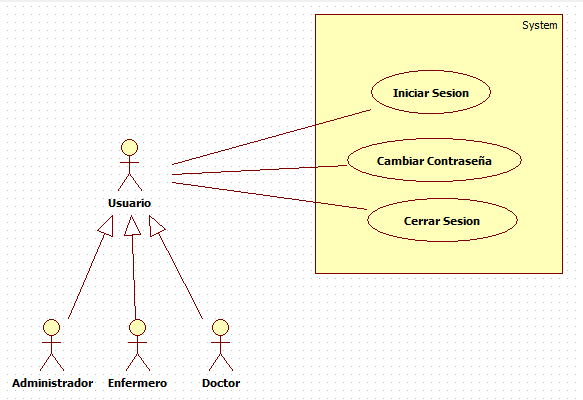
\includegraphics{../imgs/casos-uso/1.png}
			\caption{CU-1 Seguridad}
		\end{figure}
		
	\newpage
		
		\begin{figure}[ht!]
		    \centering
			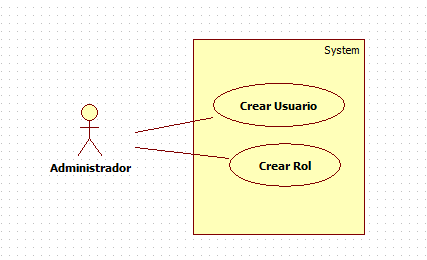
\includegraphics{../imgs/casos-uso/2.png}
			\caption{CU-2 Creación de Usuarios}
		\end{figure}
		
		\begin{figure}[ht!]
		    \centering
			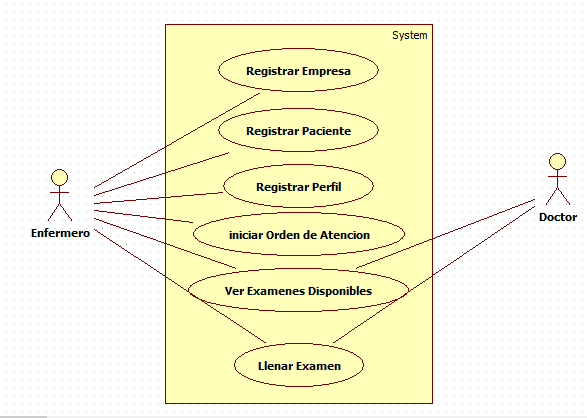
\includegraphics{../imgs/casos-uso/3.png}
			\caption{CU-3 Casos de Uso primordiales}
		\end{figure}
		

	\newpage
	\section{Diseño del Sistema}
		A continuación se muestra parte del diagrama de clases y el diagrama de
		procesos (BPM):\footnote{Se puede encontrar los diagramas completos y legibles
		en
		\href{https://www.github.com/w11ld33r/informe-practicas/tree/master/imgs}{https://www.github.com/w11ld33r/informe-practicas/tree/master/imgs}}

		\begin{figure}[H]
		    \centering
			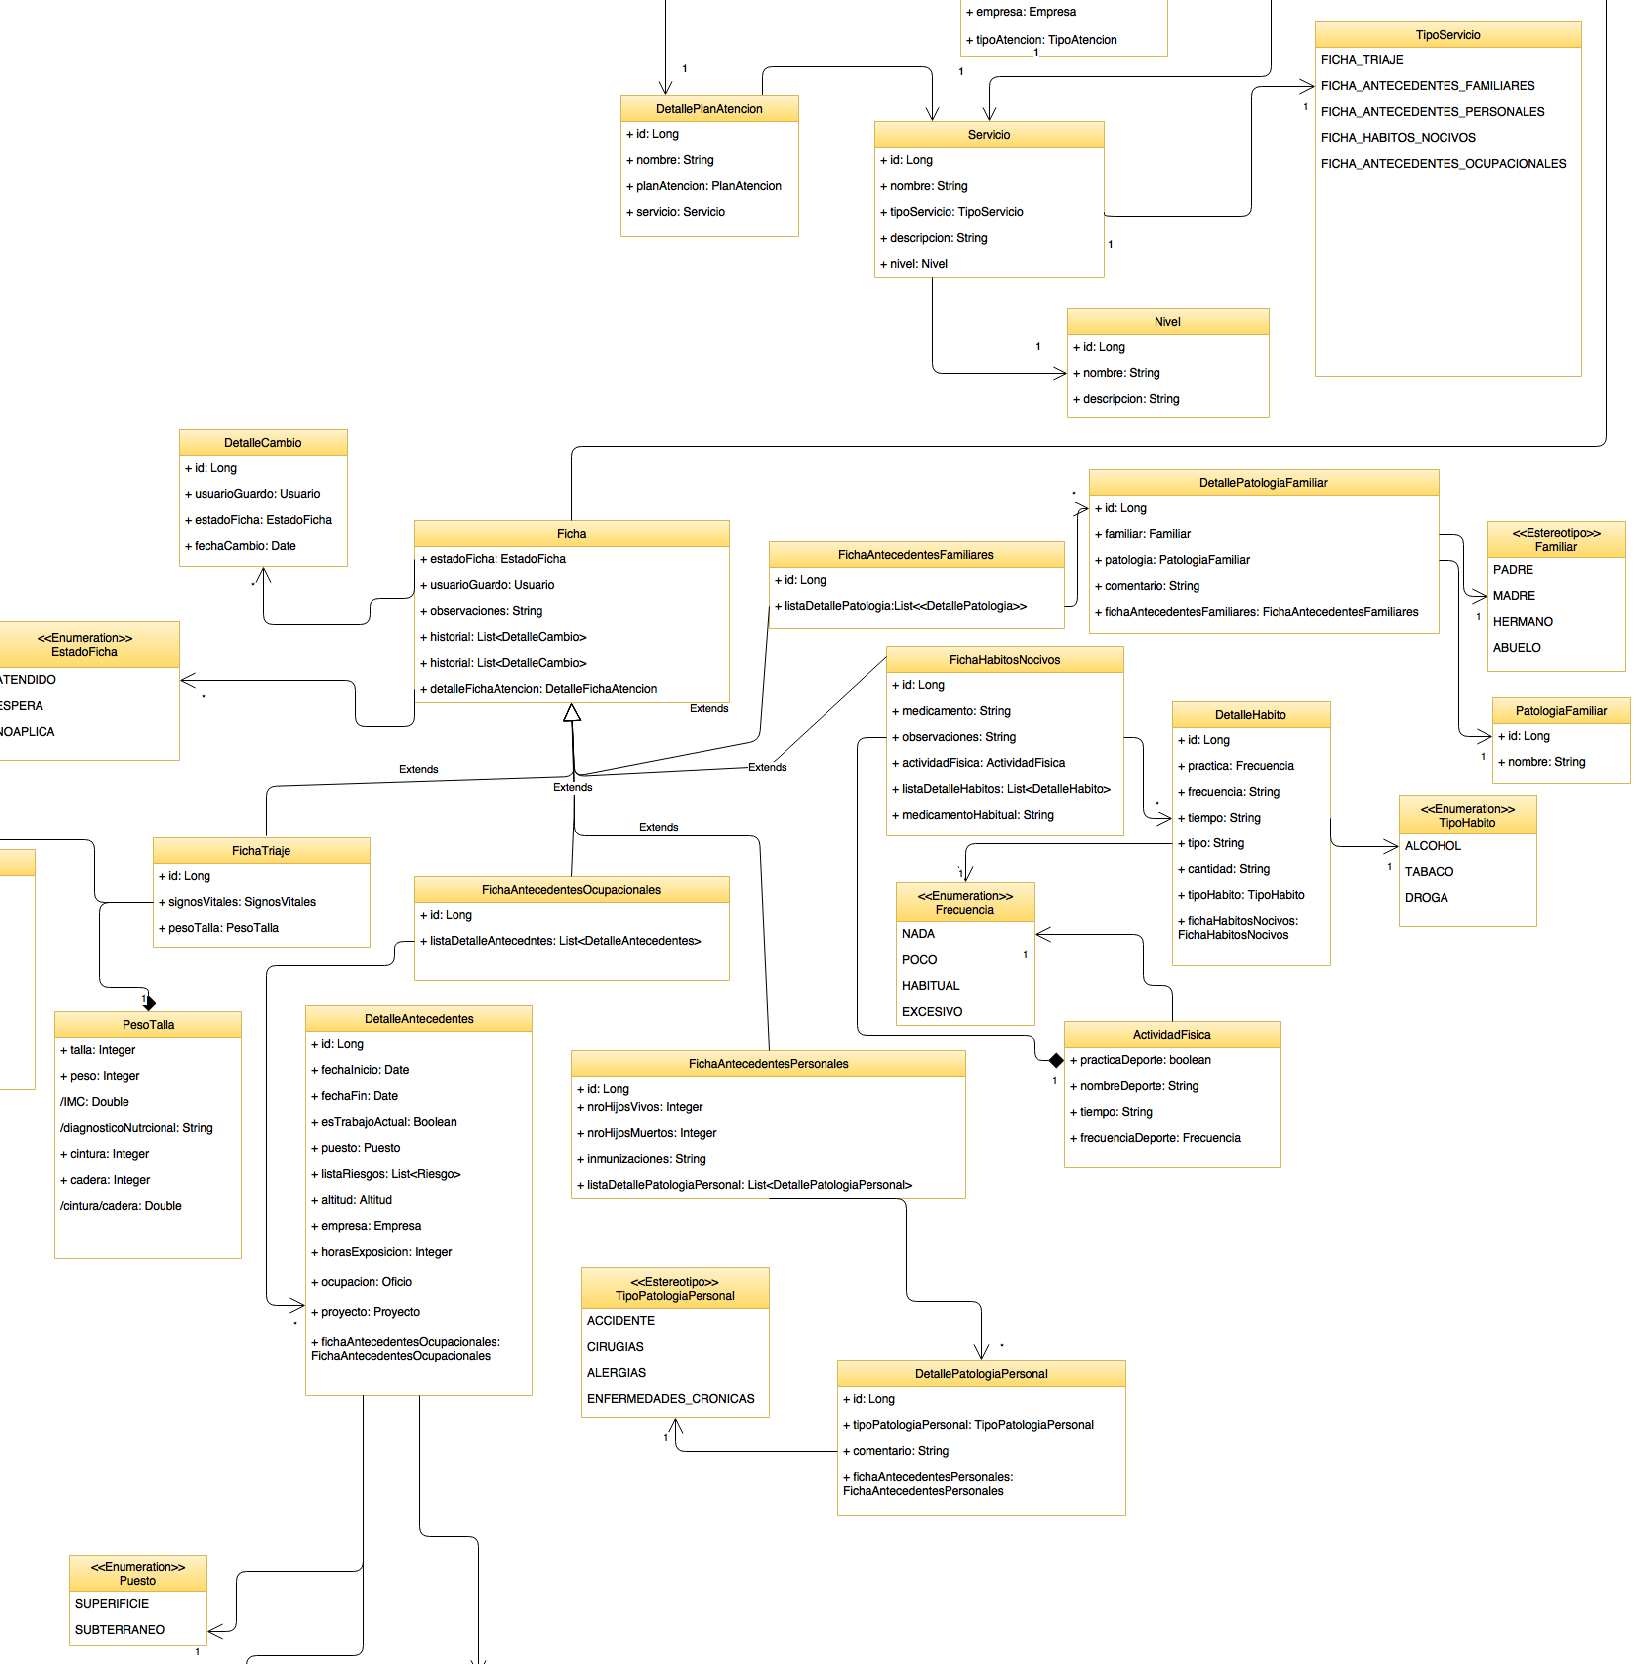
\includegraphics[width=17cm]{../imgs/disenio/DC2.png}
			\caption{DC-A Diagrama de clases}
		\end{figure}
		\begin{figure}[H]
		    \centering
			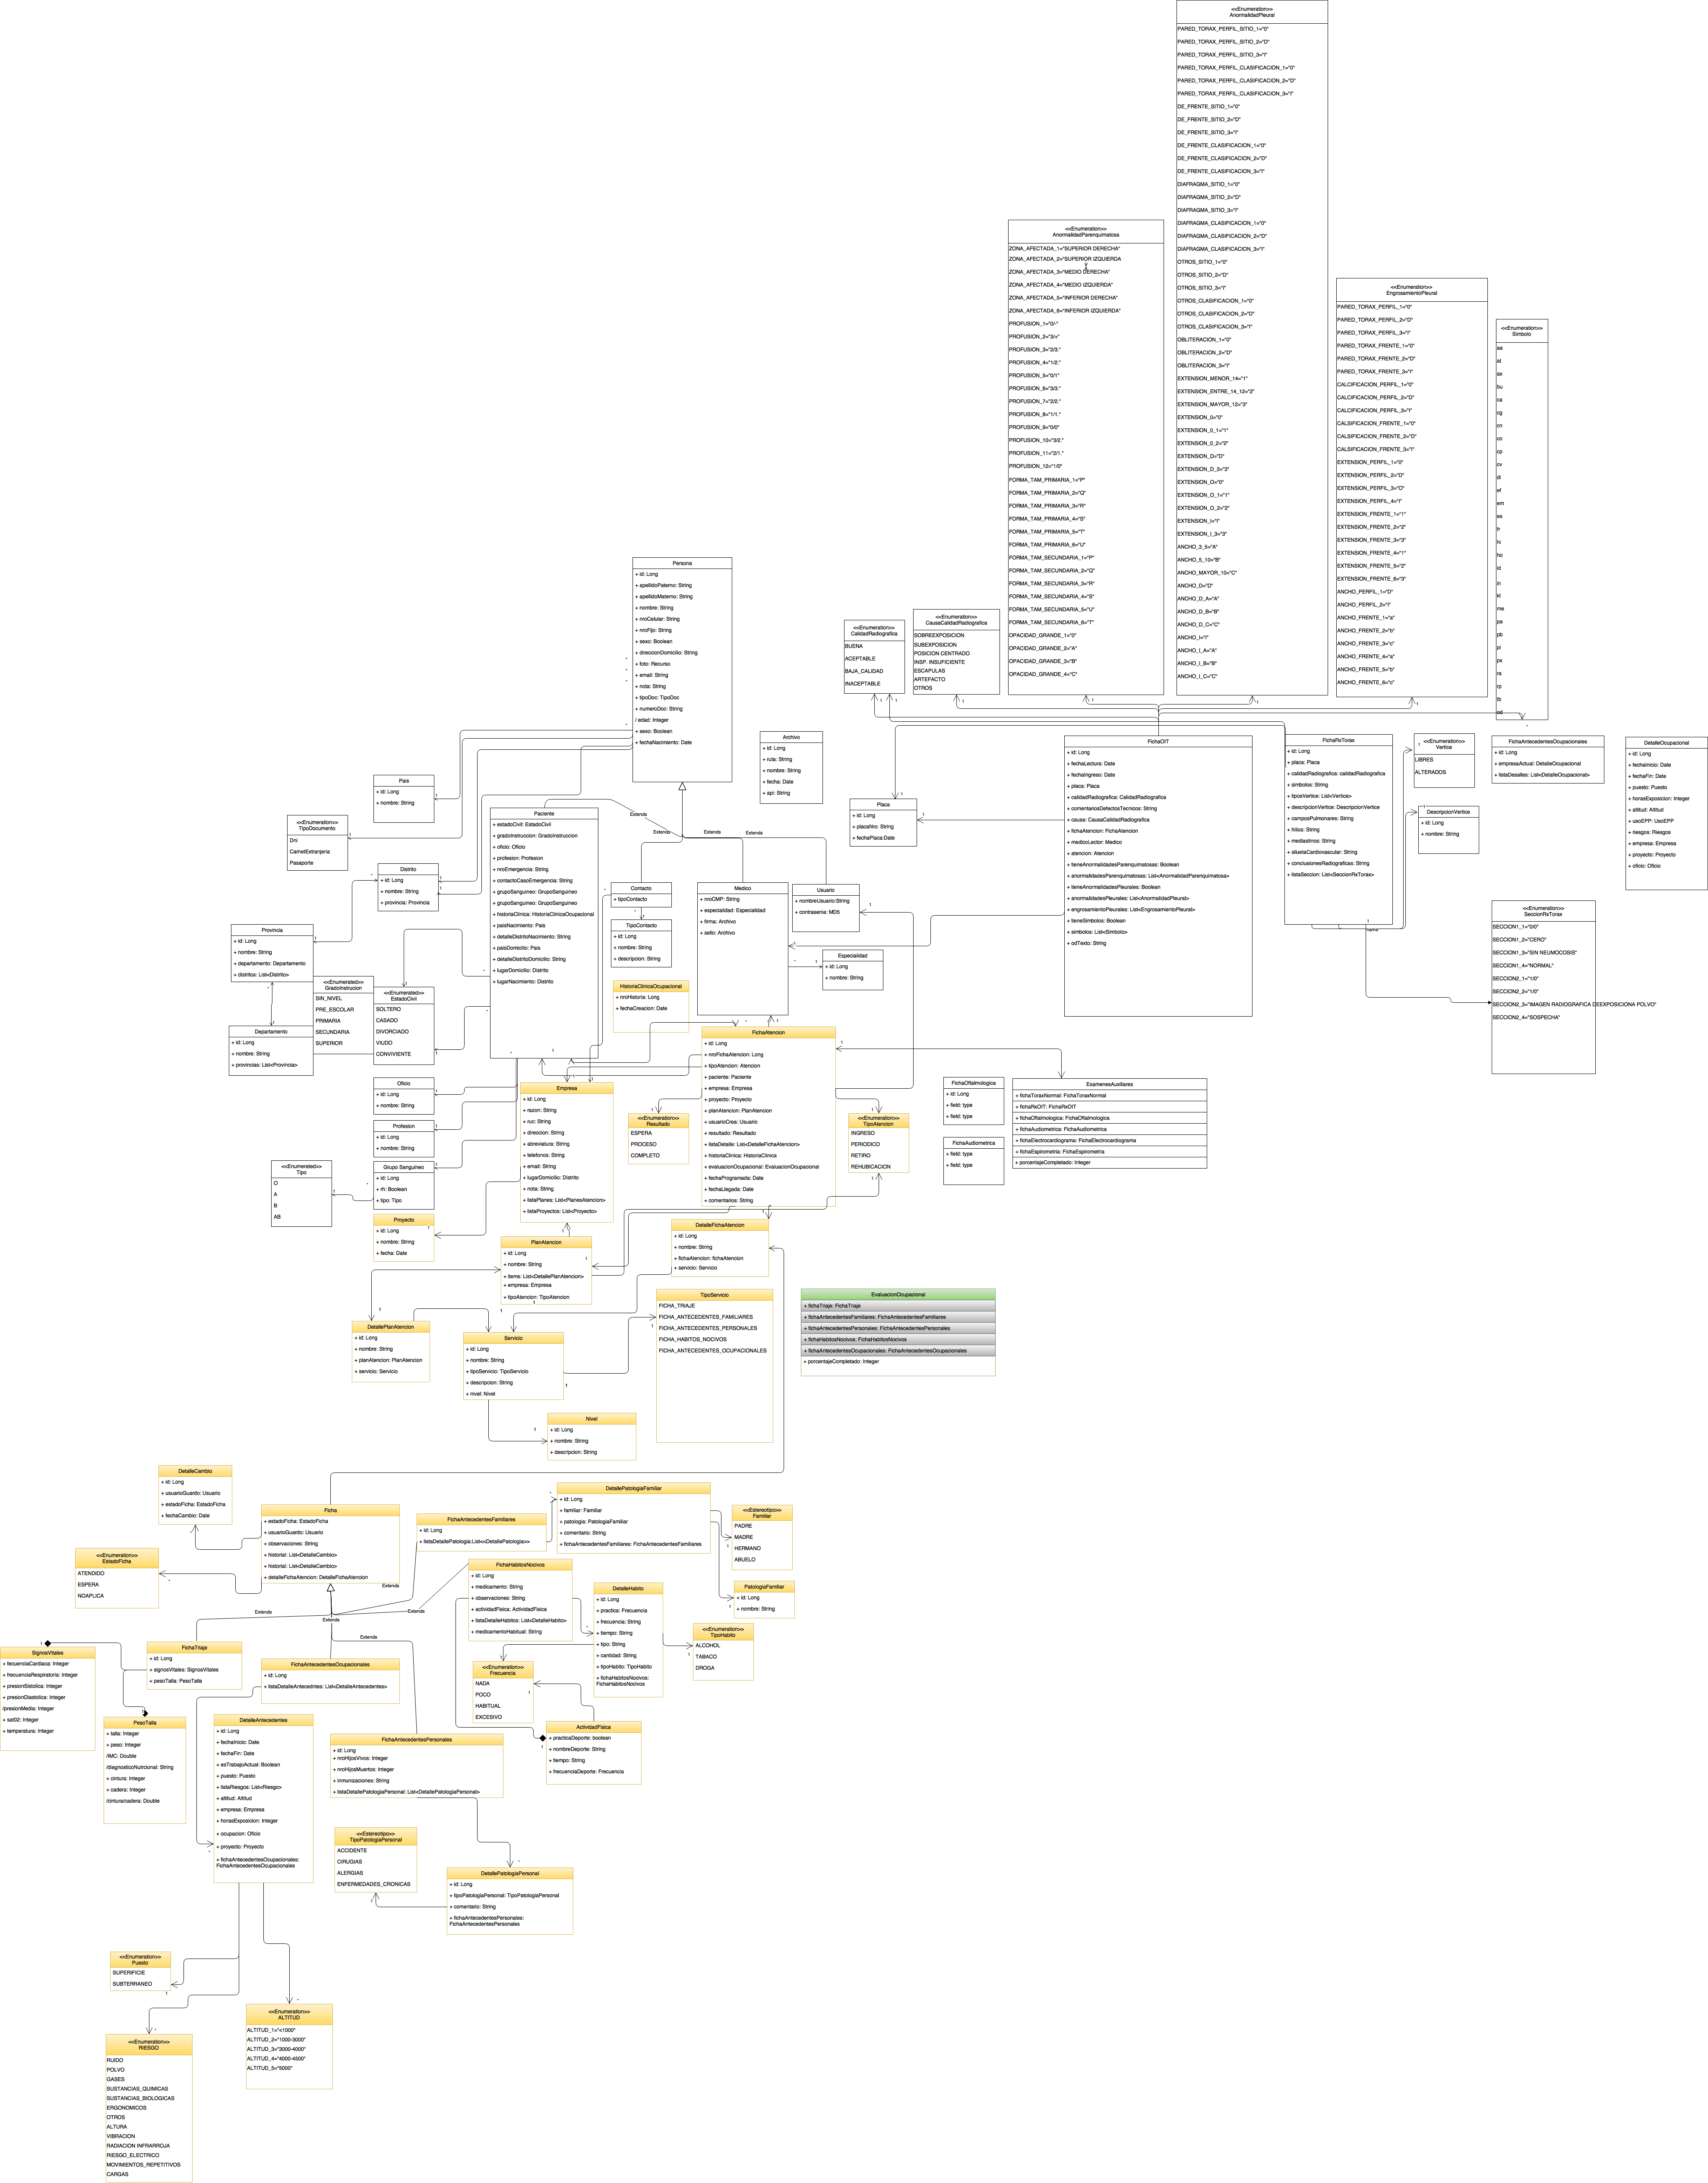
\includegraphics[width=18cm]{../imgs/disenio/DC.png}
			\caption{DC-B Diagrama de clases completo}
		\end{figure}
		\begin{figure}[H]
		    \centering
			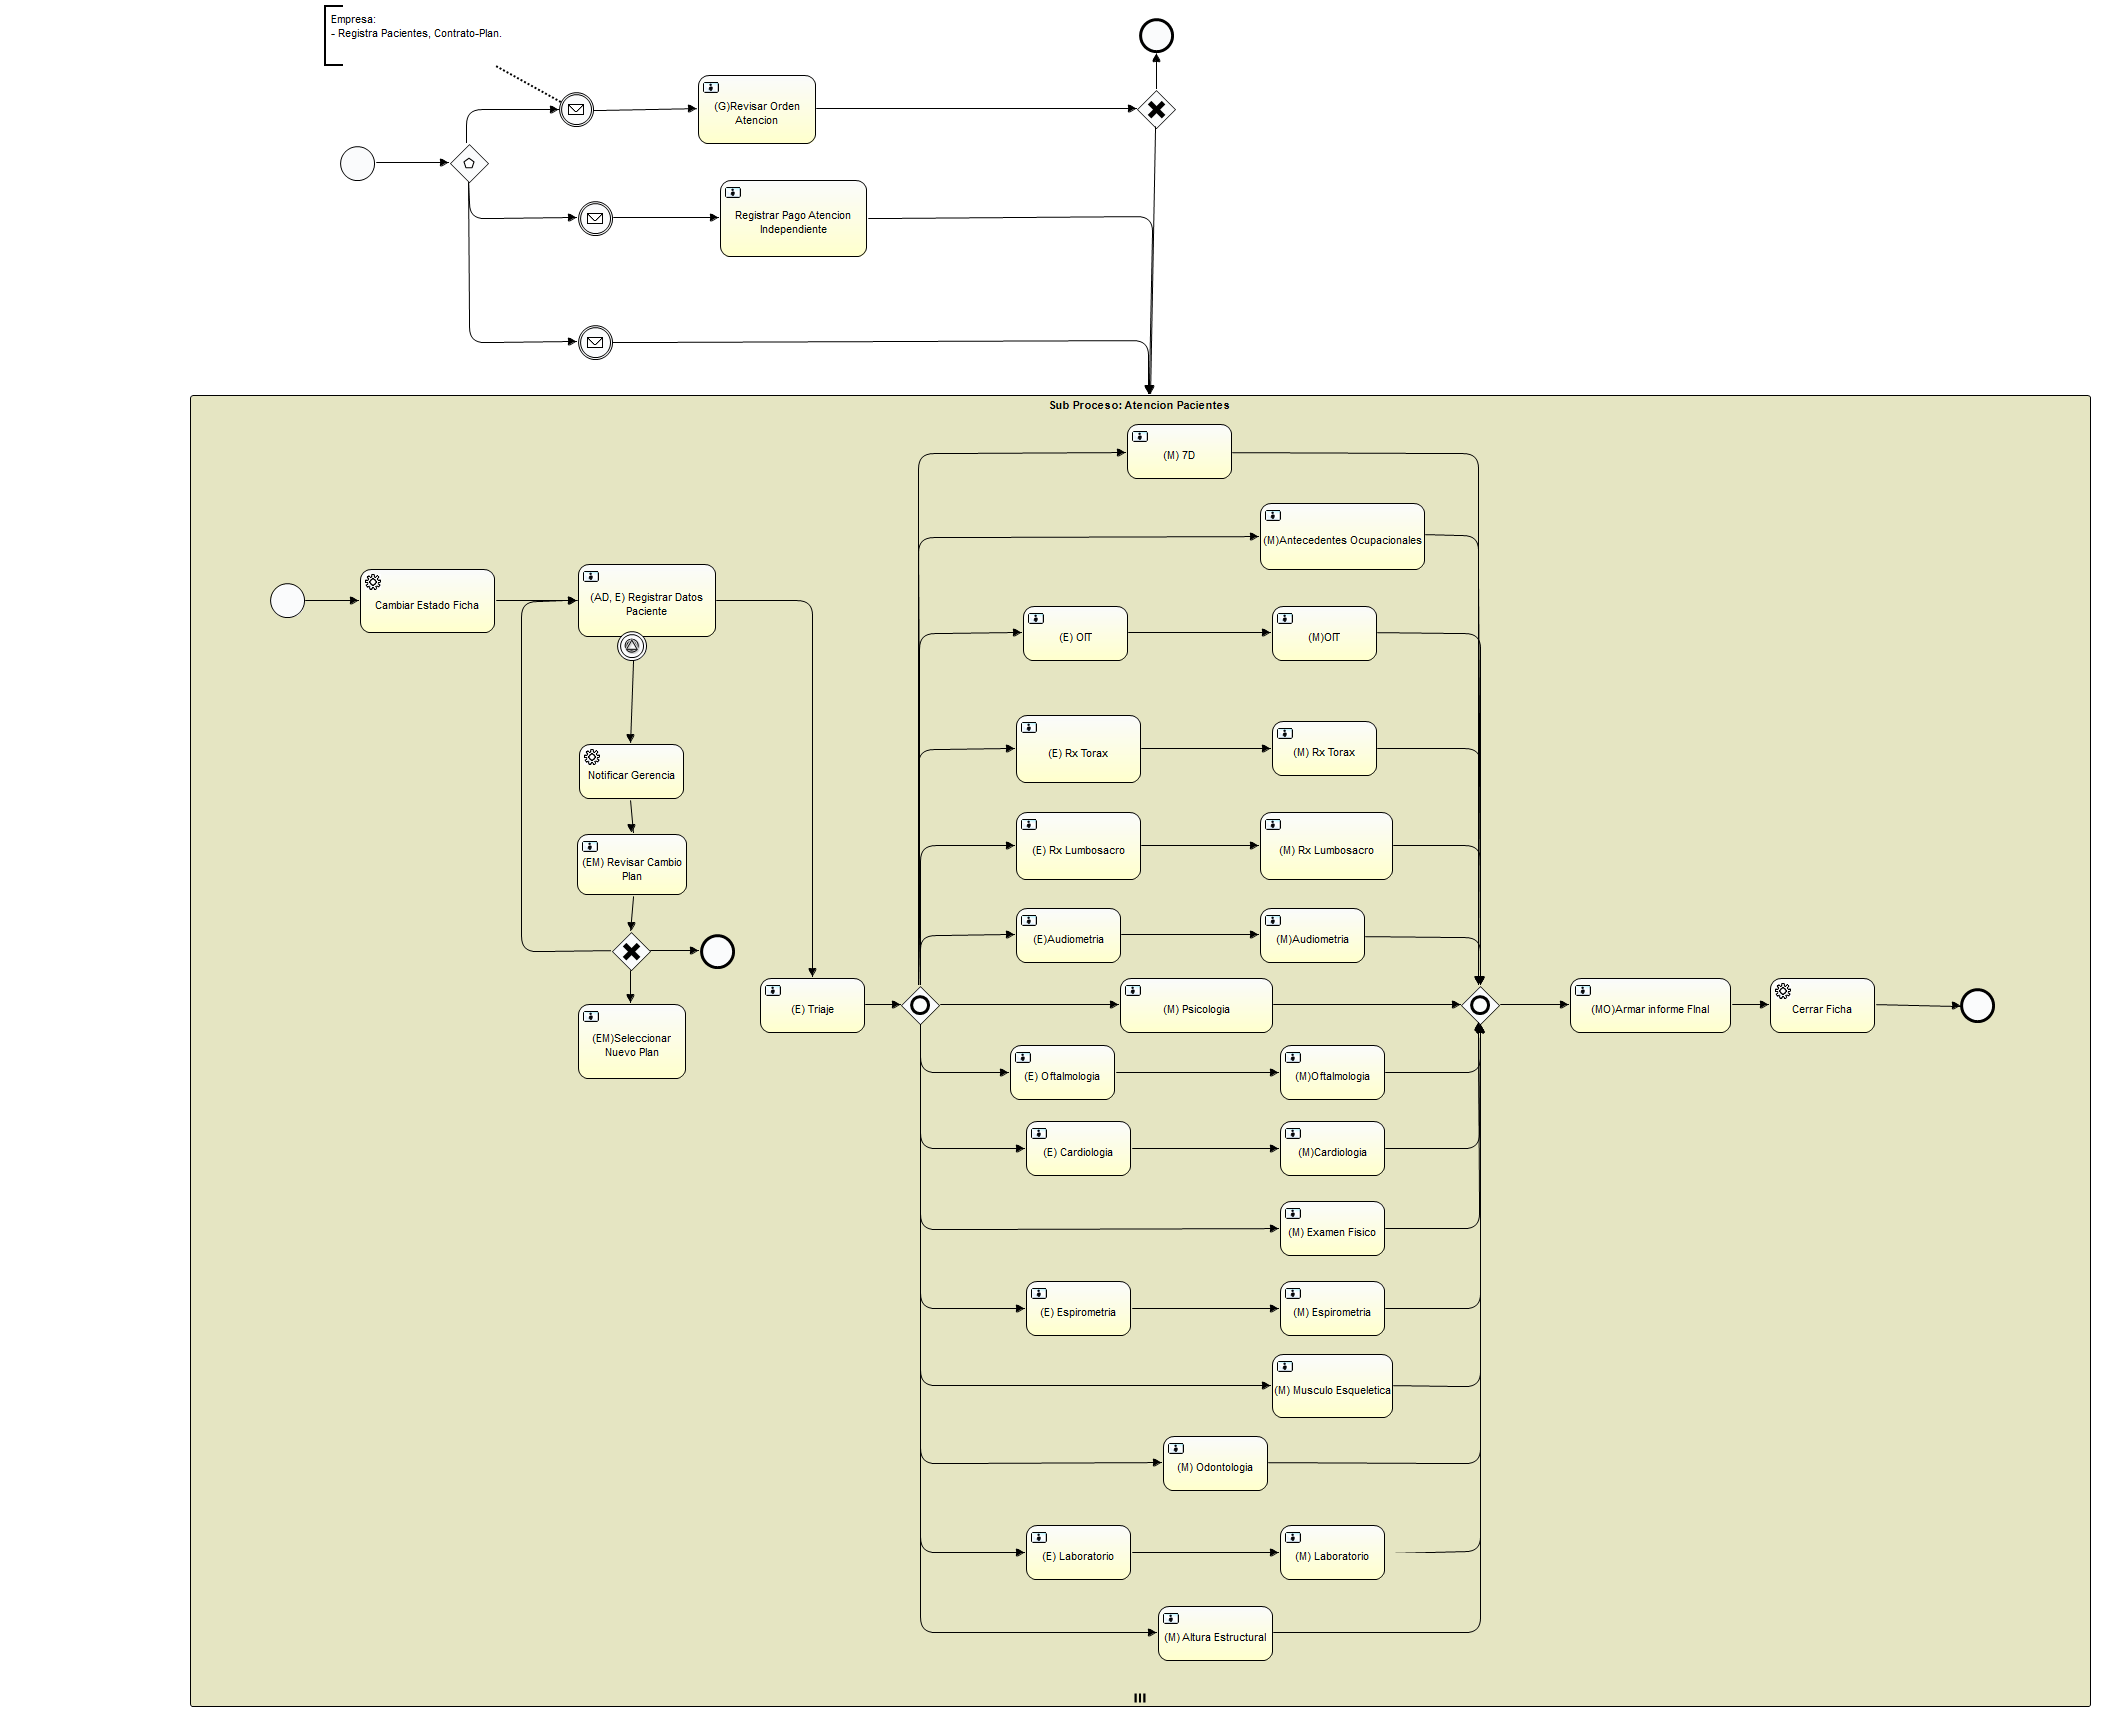
\includegraphics[width=18cm]{../imgs/disenio/ProcesoAtencion.png}
			\caption{DP-1 Diagrama BPM}
		\end{figure}
	\newpage
	\section{Arquitectura del Sistema}
	
		El Sistema sigue una arquitectura REST (Representational state trasfer) ó
		de servicios web RESTful cliente-servidor que, funciona bajo el protocolo
		HTTP, figura \ref{figure:arq1}. Básicamente el backend se encarga 
		de proporcionar recursos (previa autorización) al frontend.
		\\\
		
		\begin{figure}[ht!]
		    \centering
			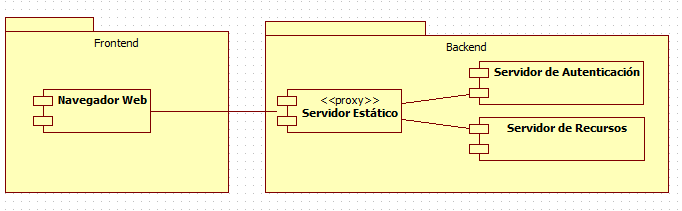
\includegraphics[width=18cm]{../imgs/disenio/arq1.png}
			\caption{DA-1 Arquitectura del Sistema}
			\label{figure:arq1}
		\end{figure}
		
		
		En la figura \ref{figure:arq2} se muestra detalladamente la interacción de los
		componentes (frontend y backend).
		\\\
		
		\begin{figure}[ht!]
		    \centering
			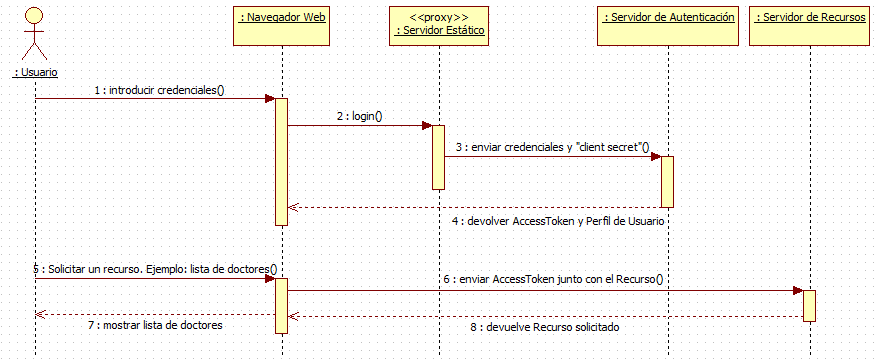
\includegraphics[width=18cm]{../imgs/disenio/arq2.png}
			\caption{DA-2 Arquitectura del Sistema (Diagrama de secuencia)}
			\label{figure:arq2}
		\end{figure}			
		
	\section{Desarrollo del Sistema}
		
		Para el desarrollo del sistema se utilizó el siguiente stack de tecnologías
		(frontend y backend):
		
		\begin{itemize}
		  \item HTML y CSS (Bootstrap)
		  \item Javascript (AngularJS)
		  \item NodeJS (ExpressJS)
		  \item Java (Spring y Spring Boot)
		\end{itemize}
		
		\subsection{Bootstrap}
			Bootstrap es un framework CSS que, facilita la creación se sitios web
			Responsive Web Design. Bootstrap viene con un conjunto de componentes de
			interfaz web listos para usar y una guía de estilos bastante completa,
			también provee grillas para el correcto maquetado de una web profesional.
			
			\begin{figure}[H]
			    \centering
				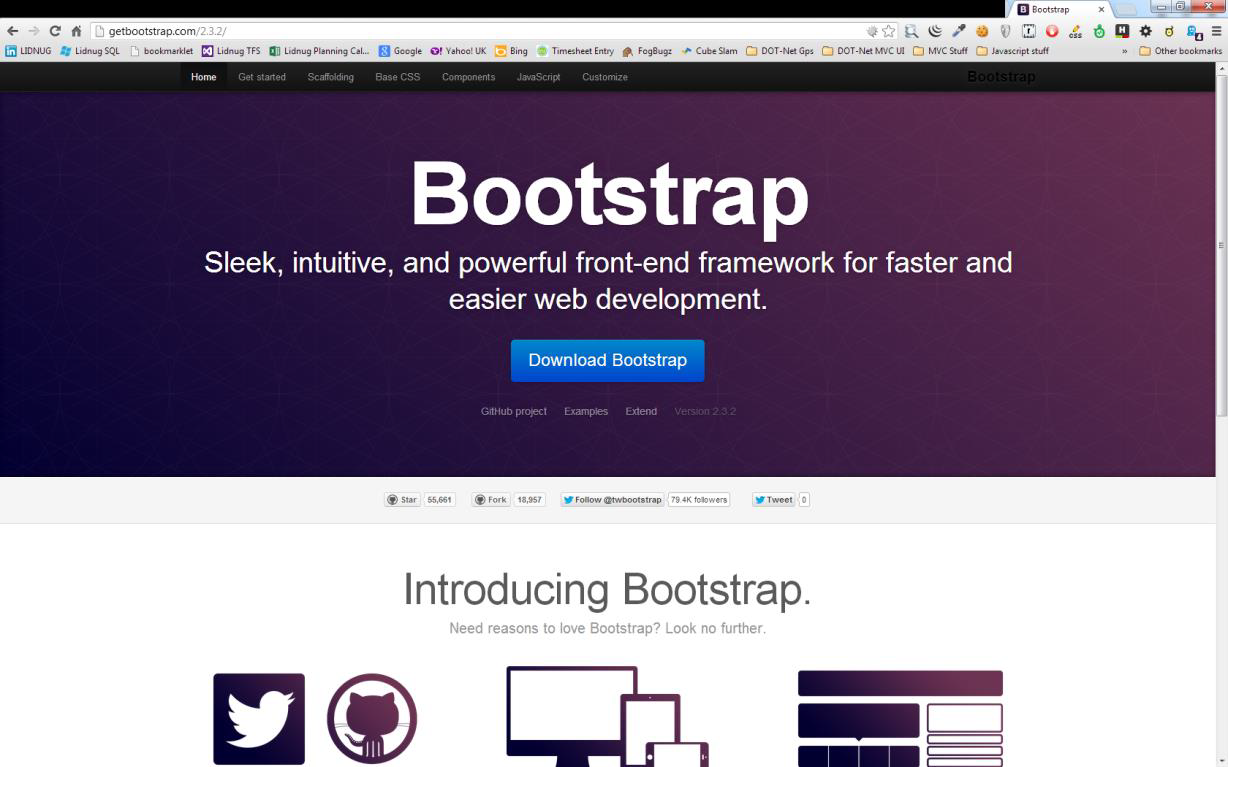
\includegraphics[width=17cm]{../imgs/ejemplos/bootstrap.png}
				\caption{Sitio Web de Bootstrap}
			\end{figure}
			
		
		\subsection{AngularJS}
			AngularJS es un framework de código abierto, soportado por Google. AngularJS
			permite a los desarrolladores crear aplicaciones web SPA (Single Page Applications), lo
			que facilita la experiencia de usuario, al no tener que cargar la
			aplicación web completa dos ó más veces.\\\
			
			A diferencia del las aplicaciones web SPA, en las aplicaciones
			web tradicionales (como se ilustra en la figura
			\ref{figure:carga-tradicional}), un cliente web hace una petición al servidor
			y éste responde con toda la página web completa; luego, el usuario hace click
			en un enlace interno, el servidor vuelve a cargar la página web completa
			y se produce un retraso en la carga de la página, lo que produce una mala
			experiencia de usuario.\footnote{Fuente de la imagen:
			\href{https://www.codeschool.com/course/shaping-up-with-angularjs}
			{https://www.codeschool.com/course/shaping-up-with-angularjs}} \\\
			
			\begin{figure}[H]
			    \centering
				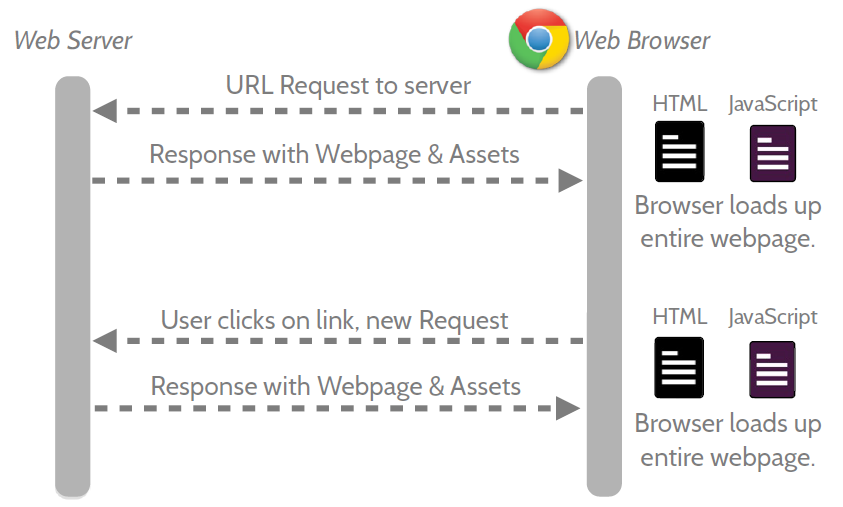
\includegraphics[width=18cm]{../imgs/ejemplos/1.png}
				\caption{Carga de página tradicional}
				\label{figure:carga-tradicional}
			\end{figure}
			
			\newpage
			
			En las aplicaciones SPA, el cliente solicita una web y el servidor
			inicialmente sirve la aplicación web completa (una sola vez); luego, el
			usuario hace click en un enlace interno, el servidor solo responde con el recurso
			solicitado, más no con la página web completa. En la figura
			\ref{figure:carga-spa} se muestra esta interacción.\footnote{Fuente de la imagen: 
			\href{https://www.codeschool.com/course/shaping-up-with-angularjs}
			{https://www.codeschool.com/course/shaping-up-with-angularjs}}
			
			\begin{figure}[H]
			    \centering
				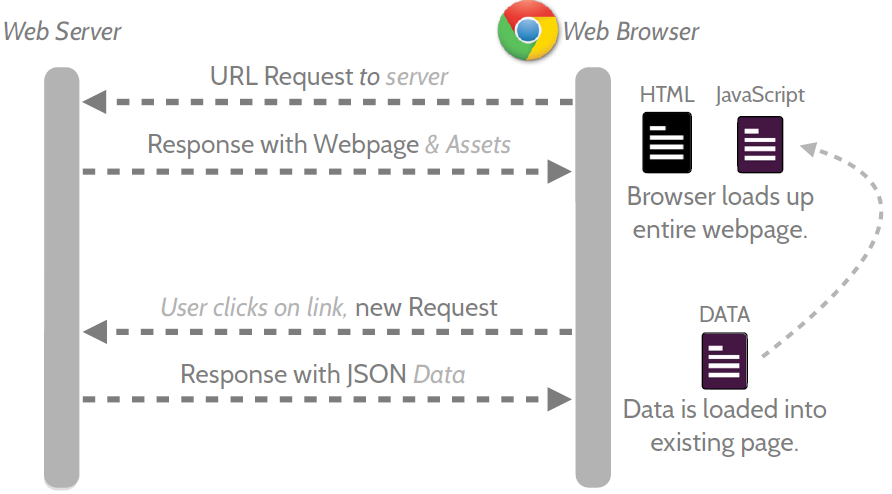
\includegraphics[width=18cm]{../imgs/ejemplos/2.png}
				\caption{Carga de página SPA}
				\label{figure:carga-spa}
			\end{figure}
			
		\subsection{NodeJS y ExpressJS}
			NodeJS no es un lenguaje de programación, es una plataforma capaz de ejecutar
			aplicaciones complejas escritas en Javascript; se ejecuta en el lado del
			servidor como cualquier otro lenguaje (Java, Python, Ruby, etc).
			Para el sistema fue usado como un proxy, y a la vez como un servidor estático.\\\
			
			ExpressJS es un framework web para NodeJS. Proporciona una API sencilla de
			utilizar, y agiliza el desarrollo de proyectos backend.
		\newpage
		
		\subsection{Spring y Spring Boot}
			Spring es un framework java para el desarrollo de aplicaciones a nivel
			empresarial, inició como una alternativa liviana al estándar {\bf Java
			Enterprise Edition (JEE)}. Spring ofrece características como inyección de
			dependencias y un modelo de programación orientada a aspectos.\\\
			
			Spring brinda muchas facilidades a la hora de programar, pero la
			configuración es un tanto compleja. Spring Boot simplifica toda las
			configuraciones iniciales para comenzar un proyecto web de manera rápida.
			Cabe mencionar que Spring Boot no es una herramienta ni una alternativa a Spring,
			es un proyecto que necesita de Spring para facilitarnos la vida.\\\
			
			Spring Boot trae algo de magia al desarrollo de aplicaciones con Spring.
			Existen cuatro características fundamentales:
			
			\begin{itemize}
			  \item {\bf Configuración Automática:} {Spring Boot proporciona de manera
			  automática funcionalidades a nuestro proyecto.}
			  
			  \item {\bf Dependencias Iniciales:} {De acuerdo al tipo de proyecto, Spring
			  Boot facilita las librerias necesarias para iniciar un proyecto.}
			  
			  \item {\bf Interfaz de Línea de Comandos:} {Esta característica opcional
			  permite escribir trozos de código directamente en la terminal e ir
			  probando funcionalidades.}
			  
			  \item {\bf Actuador (\textit{The Actuator}):} {Muestra características de
			  una aplicación en tiempo de ejecución.}
			\end{itemize}
			
		
		
		
		
		
		
		
		
